\documentclass{article}

\usepackage{fontspec}
\usepackage{fullpage}
\usepackage{multicol}
\usepackage{multirow}
\usepackage{tikz}

\begin{document}

\newfontfamily\swfill{SuttonSignWritingFill.ttf}
\newfontfamily\swline{SuttonSignWritingLine.ttf}
\newcommand{\bul}{\hfil$\bullet$&}
\renewenvironment{glossary}{\begin{multicols}{5}\begin{center}}{\end{center}\end{multicols}}
\setcounter{secnumdepth}{0}
\setlength{\columnseprule}{1pt}

\section{Supplement For Lesson 5}

\begin{center}
\it
Objectives inspired by, vocabulary transcribed from, and sentences and story by Bill Vicars.

Handshape photos by Adam Frost.

No endorsement implied nor given by either.
\end{center}

\subsection{Objectives}

\begin{tabular}{p{1cm}p{14cm}}
\bul I have completed the objectives for this lesson.\\
\bul I understand how SignWriting handles eye-gaze and roles.\\
\bul I am able to read the numbers 30--99.\\
\bul I am able to show the meaning and form of the symbol groups in the faces category in order.\\
\bul I understand the types of handshapes which are in Symbol Groups eight, nine, and thumb.\\
\bul I am able to draw the cup palmshape in all forms.\\
\bul I am able to draw and demonstrate what fill four means.\\
\bul I am able to read, write, and the ASL handshapes in symbol group three.\\
\bul I am able to recognize the vocabulary for this lesson.\\
\bul I am able to read the practice sentences for this lesson.\\
\bul I am able to read the practice story for this lesson.\\
\end{tabular}

\subsection{SignWriting Lanes}

In most SignWriting the words are centered in columns, but in the story for lesson four you may have noticed that some portions of the sentence were off center.
When SignWriting is written in a column on the right, it refers to the speaker turning to the right to sign to or for the imaginary person identified in that space, with a similar meaning when the words are in a column to the left.

In live signing you can technically have any number of roles in a particular conversation --- memory permitting.
So a person could turn to the right a little for one person and turn fully to the right for a second person, and have two more people on the left, mabye take a step forward for another person, $\ldots$.
There are SignWriting symbols which allow for the full expression of all the different roles one could take like: B521x521S38000480x480, B521x521S38011480x480, B521x521S38022480x480, and B521x521S38033480x480.
So, to refer to someone on the far right you could use B521x521S37f36480x480 followed by the phrase being signed for/to that person followed by B521x521S37f00480x480 to indicate a return to normal signing space.

But roles are such an intrinsic part of signing that this is too cumbersome for conversational SignWriting, so in conversational SignWriting ---
and by conversational we not only mean the SignWriting used on a daily basis by native ASL speakers but also the SignWriting that you are learning ---
two roles are supported and some sentences may require adjustment to fit within this framework.

This should not be surprising, it is no different than adding ``he said'' and ``she said'' to written sentences in English instead of just modulating our voice when just speaking.
My \emph{exact words} might by ``I knew Bill was there so I knocked on the door. What are you doing at my house?'' and the difference in my voice clearly indicates that I went to Bill's house and he asked the question.
The words are ambiguous, I could have gone to my house and asked Bill why he was there, but a change in voice can indicate something different.
But when I write this down what I write is ``I knew Bill was there so I knocked on the door. He asked me `what are you doing at my house?'\,''

\begin{center}
R545x518S2ff00482x483S18510520x491S18518453x492S26a00517x472S26a10461x473S2fb00492x461
M545x518S2ff00482x483S18510520x491S18518453x492S26a00517x472S26a10461x473S2fb00492x461
L545x518S2ff00482x483S18510520x491S18518453x492S26a00517x472S26a10461x473S2fb00492x461
\end{center}

Means when the person on the right said teach, I said/say teach, and the person on the left said teach.

These lanes can also be used to increase the number of people being referred to in a single conversation.

\begin{center}
L521x519S10041500x489S26501480x481
M521x519S10041500x489S26501480x481
M509x523S10040494x493S26500492x477
M515x519S10047485x498S26507501x481
R515x519S10047485x498S26507501x481
\end{center}

Though, we will try and avoid referring to that many people or places in a single conversation.

\subsection{The Numbers 31 through 99}

In \emph{general} just place the individual digits in a row.
Sometimes when writing short numbers, you may write them vertically especially if you are copying down numbers as seeing them.
Both of the following are acceptable ways to write the number 38.

\begin{center}
\begin{tabular}{*{3}{c}}
B512x515S11e20489x485&\ \ \ \ \ &B523x515S11e20477x485S1bb20502x487\\
B511x514S1bb20490x486\\
\end{tabular}
\end{center}

You may even find names fingerspelled horizontally this way, just like you would capitalize a person's name in English.

In page numbers and other similar contexts you will also find the numbers 10--29 written horizontally as individual digits even though it is bad signing.
The real reason it's acceptable for page numbers is because it simplifies typesetting, but don't sign that way even though you will see it on documents made by native signers on \texttt{http://www.signwriting.org}!

\subsection{The Faces Category}

We informally call this category faces, though it's official name is ``Head \& Face'' and has five categories in it.

\begin{center}
\begin{tabular}{ccp{21mm}c@{\hskip 5mm}ccp{21mm}c}
\textbf{Symbol}&&&&\textbf{Symbol}\\
\textbf{Group}&\textbf{Name}&\textbf{Meaning}&\textbf{Example}&\textbf{Group}&\textbf{Name}&\textbf{Meaning}&\textbf{Example}\\
\textbf{22}&Head  &The whole head.&B518x518S2ff00482x483&\textbf{23}&Eyes &Above the nose.&B518x518S30a00482x483\\
\textbf{24}&Middle&Ears and nose. &B518x518S32a00482x483&\textbf{25}&Mouth&Teeth and lips.&B518x518S33b00482x483\\
\textbf{26}&Tongue&Inside mouth.  &B518x518S35900482x483\\
\end{tabular}
\end{center}

These symbol groups constitute the bulk of the last set of ten symbol groups and they mostly move from hte top of the head down.
The symbol group tongue also has a few extras like neck, hair, and excitement but is still part of the tongue symbol group.

\subsection{Symbol Groups Eight, Nine, and Thumb}

The eighth Symbol Group we informally call eight, though it's official name is ``Middle Finger''.
Symbol Group Middle Finger (Eight) has all the handshapes where either the middle finger is extended or all fingers except the middle finger are extended.

The ninth Symbol Group we informally call nine, though it's official name is ``Index Thumb''.
Symbol Group Index Thumb (Nine) has all the handshapes where either the index finger and thumb are extended or everything except the index and thumb are extended.
This consideration of the thumb is very different from the prior three symbol groups and is helpful to remember when trying to find an unfamiliar handshape.
It is also why many of these handshapes are not part of symbol group one even though you may think to look there as well.

The tenth Symbol Group we informally call thumb, and it's official name also happens to be ``Thumb''.
Symbol Group Thumb have all the handshapes where the only modifier from fist is thumb, as well as the remaining fist shapes.

Before you can consider this lesson complete, you need to be able to list off the symbol grops as:
``one, two, three, four, five, six, seven, eight, nine, thumb.''

You may find yourself accidentally called the tenth symbol group ten, but keep at it until you can remember that it's thumb.

\subsubsection{The Cup Palmshape}

\begin{center}
\begin{tabular}{r*{6}{c}}
&\textbf{Fill 1}&\textbf{Fill 2}&\textbf{Fill 3}&\textbf{Fill 4}&\textbf{Fill 5}&\textbf{Fill 6}\\
\multirow{3}{*}{\textbf{Right}}&
B509x510S16d00492x490&
B509x510S16d10492x490&
B509x510S16d20492x490&
B509x510S16d30492x490&
B509x510S16d40492x490&
B509x510S16d50492x490\\
&
\tikz{\draw[thick](0,0)--(0,10pt);\draw[thick](0,0)arc(270:210:5pt);\draw[thick](5pt,5pt)arc(0:-90:5pt);\draw[thick](0,10pt)arc(90:0:5pt);\draw[thick](0,10pt)arc(90:150:5pt);}&
\tikz{\draw[thick](0,0)--(0,10pt);\draw[thick](0,0)arc(270:210:5pt);\draw[thick](5pt,5pt)arc(0:-90:5pt);\draw[thick](0,10pt)arc(90:0:5pt);\draw[thick](0,10pt)arc(90:150:5pt);\draw[thick](2.5pt,9pt)--(2.5pt,1pt);}&
\tikz{\draw[thick](0,0)--(0,10pt);\draw[thick](0,0)arc(270:210:5pt);\draw[thick](5pt,5pt)arc(0:-90:5pt);\draw[thick](0,10pt)arc(90:0:5pt);\draw[thick](0,10pt)arc(90:150:5pt);\draw[thick](0,10pt)--(2.5pt,1pt);\draw[thick](0,0)--(2.5pt,9pt);}&
\tikz{\draw[thick](0,0)--(0,10pt);\draw[thick](0,0)arc(270:210:5pt);\draw[thick](5pt,5pt)arc(0:-90:5pt);\draw[thick](0,10pt)arc(90:0:5pt);\draw[thick](0,10pt)arc(90:150:5pt);\draw(-2pt,-3pt)--(-2pt,13pt);}&
\tikz{\draw[thick](0,0)--(0,10pt);\draw[thick](0,0)arc(270:210:5pt);\draw[thick](5pt,5pt)arc(0:-90:5pt);\draw[thick](0,10pt)arc(90:0:5pt);\draw[thick](0,10pt)arc(90:150:5pt);\draw[thick](2.5pt,9pt)--(2.5pt,1pt);\draw(-2pt,-3pt)--(-2pt,13pt);}&
\tikz{\draw[thick](0,0)--(0,10pt);\draw[thick](0,0)arc(270:210:5pt);\draw[thick](5pt,5pt)arc(0:-90:5pt);\draw[thick](0,10pt)arc(90:0:5pt);\draw[thick](0,10pt)arc(90:150:5pt);\draw[thick](0,10pt)--(2.5pt,1pt);\draw[thick](0,0)--(2.5pt,9pt);\draw(-2pt,-3pt)--(-2pt,13pt);}\\
\textbf{Left}&
B509x510S16d08492x490&
B509x510S16d18492x490&
B509x510S16d28492x490&
B509x510S16d38492x490&
B509x510S16d48492x490&
B509x510S16d58492x490\\
\end{tabular}
\end{center}

\subsection{The Fourth Fill}

\subsubsection{Hand Symbols}

\begin{center}
B508x515S10030493x485 B508x515S10e30493x485 B512x515S11e30489x485
\end{center}

Any symbol drawn in the fourth fill means that the signer's palm is facing up.
For all the hand symbols, the empty portion represents the signer's palm and the filled portion represents the back of the hand.
So for fill four, if the hand was open you would see all of your palm --- leaving fill four a completely empty symbol.

\subsubsection{Movement Symbols}

\begin{center}
B508x515S22b30492x485 B508x515S25630492x485 B508x515S26630492x485
\end{center}

Any movement symbol drawn in the fourth fill means that there is no arrowhead, allowing for creation of larger arrows by placing these next to any arrows in the other fills.

\subsubsection{Everything Else}

\begin{center}
B506x504S2f710494x497 B518x518S30a20482x483 B537x504S38730463x496
\end{center}

The fills for other categories tend to be a bit more variable.
Here we have an alternate form of double-fast, eyebrows raised without a face, and tense comma.

\subsection{ASL Handshapes From Symbol Group Three}

The twelve handshapes in Symbol Group Three used by ASL in order are:
Index Middle Thumb;
Index Middle Bent, Thumb Straight;
Index Middle Thumb Bent;
Index Up, Middle Hinge, Thumb Side;
Index Middle Thumb Cup;
Index Middle Thumb Circle;
{\bf
Index Middle Unit, Thumb Side;
Index Middle Unit Hinge, Thumb Side;
Index Middle Cross, Thumb Side;
Middle Thumb Circle, Index Up;
Index Middle Thumb, Angle;
and Middle Thumb Angle Out, Index Up.
}

\subsubsection{The Index Middle Unit, Thumb Side Handshape}

\begin{center}
\begin{tabular}{r*{6}{c}}
&\textbf{Fill 1}&\textbf{Fill 2}&\textbf{Fill 3}&\textbf{Fill 4}&\textbf{Fill 5}&\textbf{Fill 6}\\
\multirow{2}{*}{\textbf{Right}}&
B512x515S12d00489x485&
B512x515S12d10489x485&
B512x515S12d20489x485&
B512x515S12d30489x485&
B512x515S12d40489x485&
B512x515S12d50489x485\\
&
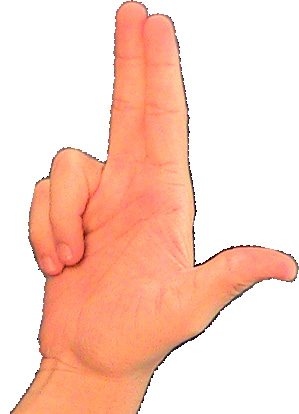
\includegraphics[scale=0.1]{images/03-07-1.jpg}&
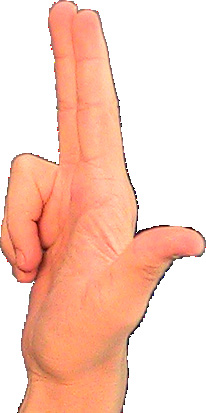
\includegraphics[scale=0.1]{images/03-07-2.jpg}&
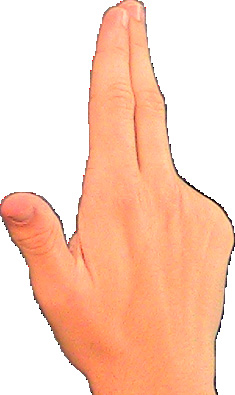
\includegraphics[scale=0.1]{images/03-07-3.jpg}&
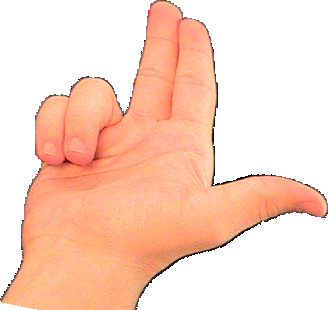
\includegraphics[scale=0.1]{images/03-07-4.jpg}&
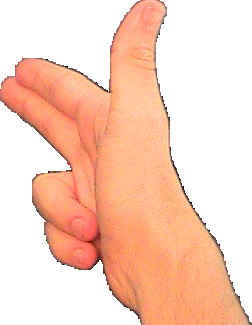
\includegraphics[scale=0.1]{images/03-07-5.jpg}&
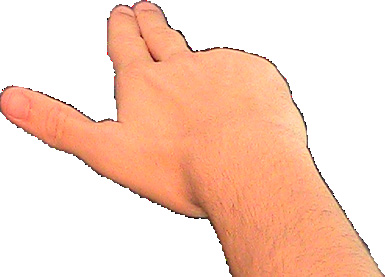
\includegraphics[scale=0.1]{images/03-07-6.jpg}\\
\textbf{Left}&
B512x515S12d08489x485&
B512x515S12d18489x485&
B512x515S12d28489x485&
B512x515S12d38489x485&
B512x515S12d48489x485&
B512x515S12d58489x485\\
\end{tabular}
\end{center}

\subsubsection{The Index Middle Unit Hinge, Thumb Side Handshape}

\begin{center}
\begin{tabular}{r*{6}{c}}
&\textbf{Fill 1}&\textbf{Fill 2}&\textbf{Fill 3}&\textbf{Fill 4}&\textbf{Fill 5}&\textbf{Fill 6}\\
\multirow{2}{*}{\textbf{Right}}&
B512x513S13200488x488&
B512x513S13210488x488&
B512x513S13220488x488&
B512x513S13230488x488&
B512x513S13240488x488&
B512x513S13250488x488\\
&
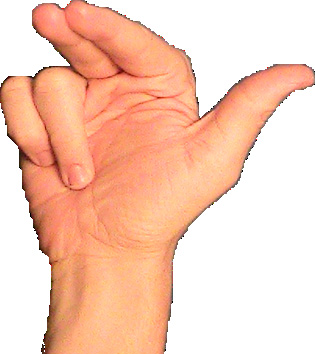
\includegraphics[scale=0.1]{images/03-08-1.jpg}&
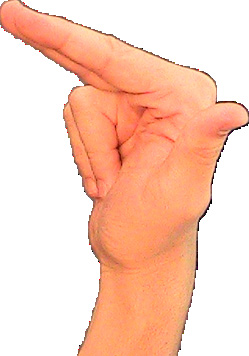
\includegraphics[scale=0.1]{images/03-08-2.jpg}&
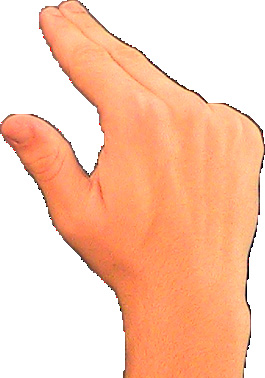
\includegraphics[scale=0.1]{images/03-08-3.jpg}&
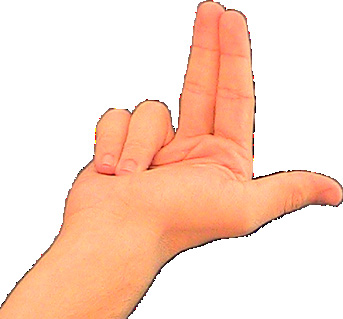
\includegraphics[scale=0.1]{images/03-08-4.jpg}&
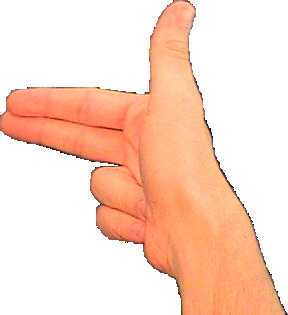
\includegraphics[scale=0.1]{images/03-08-5.jpg}&
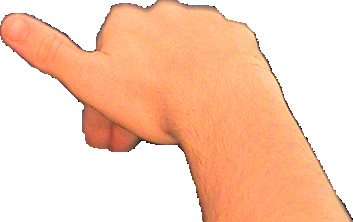
\includegraphics[scale=0.1]{images/03-08-6.jpg}\\
\textbf{Left}&
B512x513S13208488x488&
B512x513S13218488x488&
B512x513S13228488x488&
B512x513S13238488x488&
B512x513S13248488x488&
B512x513S13258488x488\\
\end{tabular}
\end{center}

\subsubsection{The Index Middle Cross, Thumb Side Handshape}

\begin{center}
\begin{tabular}{r*{6}{c}}
&\textbf{Fill 1}&\textbf{Fill 2}&\textbf{Fill 3}&\textbf{Fill 4}&\textbf{Fill 5}&\textbf{Fill 6}\\
\multirow{2}{*}{\textbf{Right}}&
B511x515S13300489x485&
B511x515S13310489x485&
B511x515S13320489x485&
B511x515S13330489x485&
B511x515S13340489x485&
B511x515S13350489x485\\
&
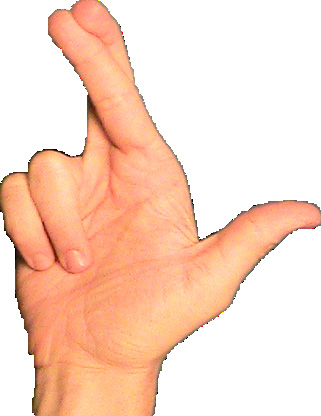
\includegraphics[scale=0.1]{images/03-09-1.jpg}&
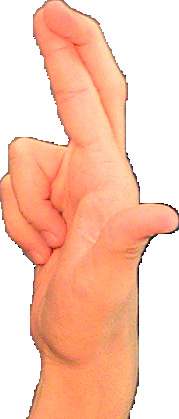
\includegraphics[scale=0.1]{images/03-09-2.jpg}&
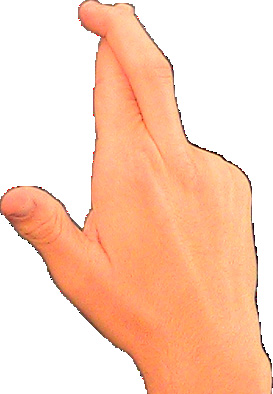
\includegraphics[scale=0.1]{images/03-09-3.jpg}&
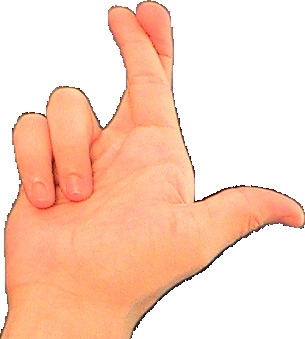
\includegraphics[scale=0.1]{images/03-09-4.jpg}&
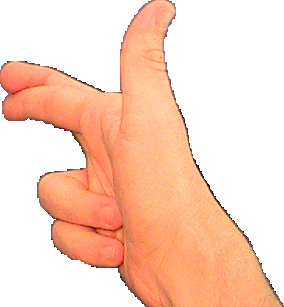
\includegraphics[scale=0.1]{images/03-09-5.jpg}&
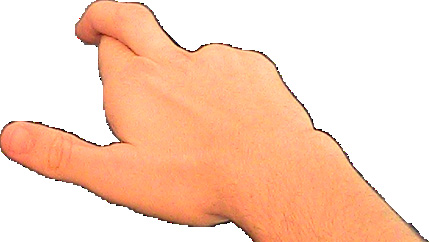
\includegraphics[scale=0.1]{images/03-09-6.jpg}\\
\textbf{Left}&
B511x515S13308489x485&
B511x515S13318489x485&
B511x515S13328489x485&
B511x515S13338489x485&
B511x515S13348489x485&
B511x515S13358489x485\\
\end{tabular}
\end{center}

\subsubsection{The Middle Thumb Circle, Index Up Handshape}

\begin{center}
\begin{tabular}{r*{6}{c}}
&\textbf{Fill 1}&\textbf{Fill 2}&\textbf{Fill 3}&\textbf{Fill 4}&\textbf{Fill 5}&\textbf{Fill 6}\\
\multirow{2}{*}{\textbf{Right}}&
B512x515S13800488x485&
B512x515S13810488x485&
B512x515S13820488x485&
B512x515S13830488x485&
B512x515S13840488x485&
B512x515S13850488x485\\
&
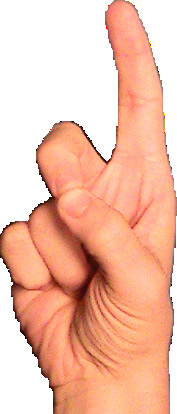
\includegraphics[scale=0.1]{images/03-10-1.jpg}&
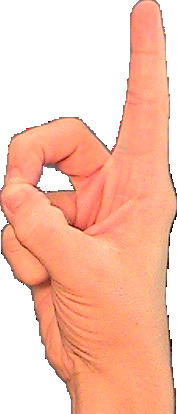
\includegraphics[scale=0.1]{images/03-10-2.jpg}&
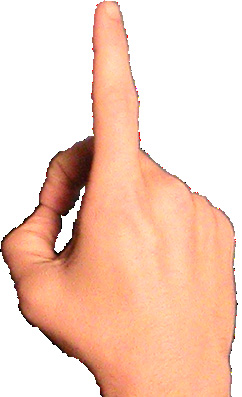
\includegraphics[scale=0.1]{images/03-10-3.jpg}&
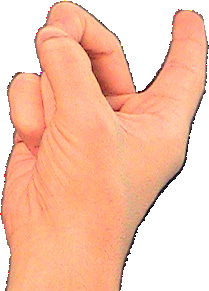
\includegraphics[scale=0.1]{images/03-10-4.jpg}&
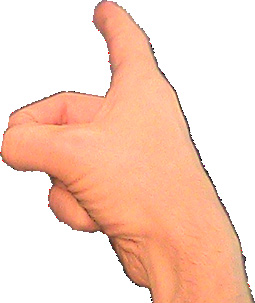
\includegraphics[scale=0.1]{images/03-10-5.jpg}&
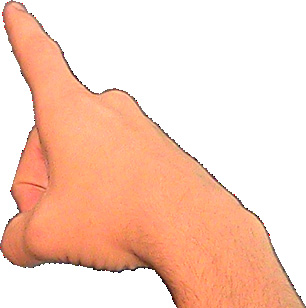
\includegraphics[scale=0.1]{images/03-10-6.jpg}\\
\textbf{Left}&
B512x515S13808488x485&
B512x515S13818488x485&
B512x515S13828488x485&
B512x515S13838488x485&
B512x515S13848488x485&
B512x515S13858488x485\\
\end{tabular}
\end{center}

\subsubsection{The Index Middle Thumb, Angle Handshape}

\begin{center}
\begin{tabular}{r*{6}{c}}
&\textbf{Fill 1}&\textbf{Fill 2}&\textbf{Fill 3}&\textbf{Fill 4}&\textbf{Fill 5}&\textbf{Fill 6}\\
\multirow{2}{*}{\textbf{Right}}&
B515x508S13f00486x493&
B515x508S13f10486x493&
B515x508S13f20486x493&
B515x508S13f30486x493&
B515x508S13f40486x493&
B515x508S13f50486x493\\
&
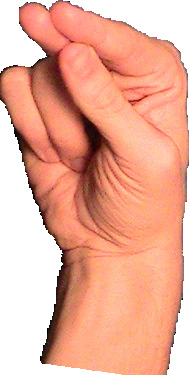
\includegraphics[scale=0.1]{images/03-11-1.jpg}&
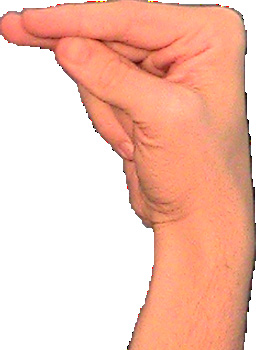
\includegraphics[scale=0.1]{images/03-11-2.jpg}&
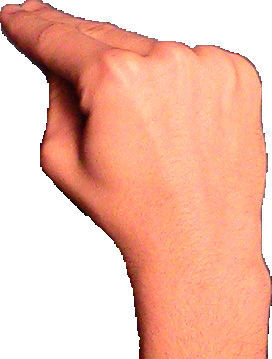
\includegraphics[scale=0.1]{images/03-11-3.jpg}&
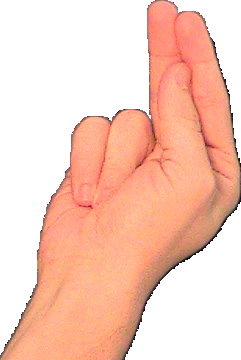
\includegraphics[scale=0.1]{images/03-11-4.jpg}&
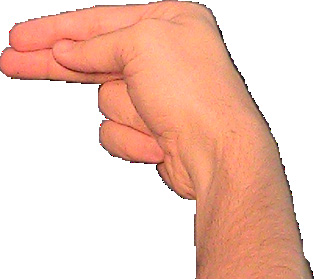
\includegraphics[scale=0.1]{images/03-11-5.jpg}&
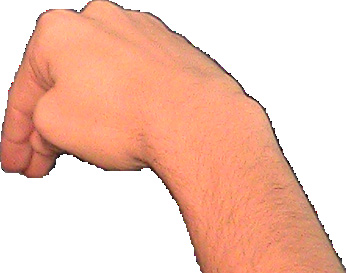
\includegraphics[scale=0.1]{images/03-11-6.jpg}\\
\textbf{Left}&
B515x508S13f08486x493&
B515x508S13f18486x493&
B515x508S13f28486x493&
B515x508S13f38486x493&
B515x508S13f48486x493&
B515x508S13f58486x493\\
\end{tabular}
\end{center}

\subsubsection{The Middle Thumb Angle Out, Index Up Handshape}

\begin{center}
\begin{tabular}{r*{6}{c}}
&\textbf{Fill 1}&\textbf{Fill 2}&\textbf{Fill 3}&\textbf{Fill 4}&\textbf{Fill 5}&\textbf{Fill 6}\\
\multirow{2}{*}{\textbf{Right}}&
B515x515S14000486x485&
B515x515S14010486x485&
B515x515S14020486x485&
B515x515S14030486x485&
B515x515S14040486x485&
B515x515S14050486x485\\
&
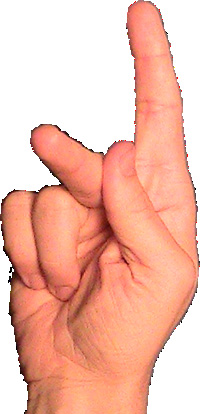
\includegraphics[scale=0.1]{images/03-12-1.jpg}&
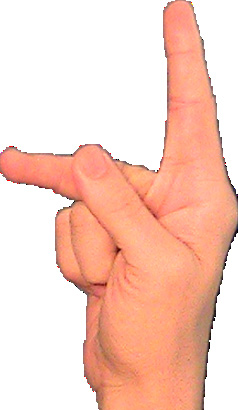
\includegraphics[scale=0.1]{images/03-12-2.jpg}&
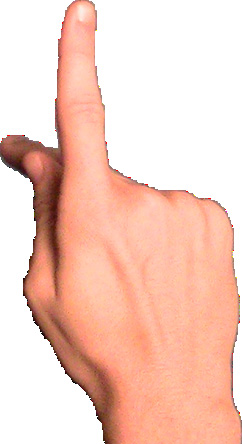
\includegraphics[scale=0.1]{images/03-12-3.jpg}&
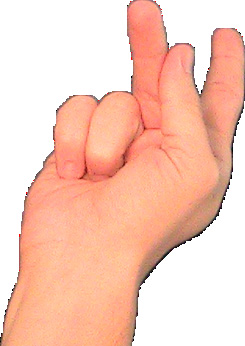
\includegraphics[scale=0.1]{images/03-12-4.jpg}&
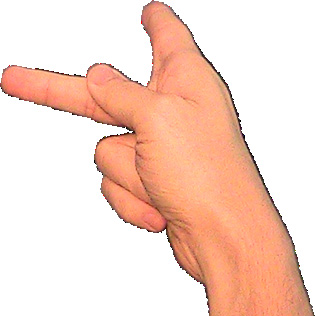
\includegraphics[scale=0.1]{images/03-12-5.jpg}&
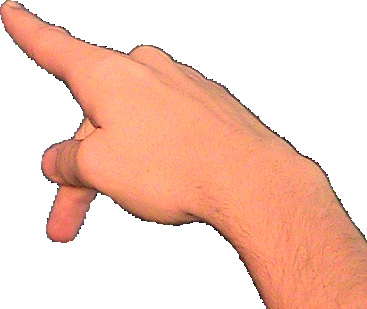
\includegraphics[scale=0.1]{images/03-12-6.jpg}\\
\textbf{Left}&
B515x515S14008486x485&
B515x515S14018486x485&
B515x515S14028486x485&
B515x515S14038486x485&
B515x515S14048486x485&
B515x515S14058486x485\\
\end{tabular}
\end{center}

\subsection{Vocabulary}

\begin{glossary}

\textbf{0}\\
AS17620M508x508S17620492x492

\textbf{can}\\
AS20350S20350S22a24M525x517S20350510x483S20350476x483S22a24494x502

\textbf{car}\\
AS20301S20301S28800S2880cS2880cS28818S28814S28818S2fb04M556x537S20301466x474S20301511x464S28800527x500S2880c510x500S2880c544x500S28814464x501S28818445x501S28818482x502S2fb04496x531

\textbf{church}\\
AS16d20S15a56S20600M523x517S15a56478x505S16d20481x483S20600501x494

\textbf{computer}\\
AS16d20S15a1aS20e00S26a02S37806M532x518S20e00485x489S16d20502x482S37806470x511S15a1a505x506S26a02469x483

\textbf{doctor}\\
AS18020S15a39S20600M527x518S15a39497x482S18020497x503S20600473x498

\textbf{drive}\\
AS20301S20301S2880cS28800S2880cS28818S28814S28814S2fb04M554x537S20301474x471S20301509x464S2880c511x503S28800527x504S2880c542x503S28814479x502S28818463x502S28814447x502S2fb04493x531

\textbf{email}\\
AS10012S16d18S26500M522x519S16d18479x494S10012492x504S26500507x482

\textbf{give}\\
AS18537S2b700M510x527S2b700491x474S18537490x500

\textbf{home}\\
AS18510S20500S22a00S20500S2ff00M530x546S2ff00482x483S18517503x519S20500493x519S22a07515x511S20500520x494

\textbf{internet}\\
AS1c510S1c518S21100S2c500S2c514S2fb00M545x535S1c510503x503S1c518467x503S2c500505x474S2c514455x473S2fb00492x465S21100494x521

\textbf{in}\\
AS18512S16d48S20710M529x524S16d48472x504S20710495x501S18512482x476

\textbf{move}\\
AS18557S1855fS2892aM533x522S18557514x479S1855f467x480S2892a486x507

\textbf{movie}\\
AS14c10S10058S20500S2a502M542x523S10058459x493S14c10482x477S20500476x501S2a502509x490

\textbf{nurse}\\
AS11920S15a39S20600M524x523S15a39501x477S11920497x497S20600477x485

\textbf{out}\\
AS14c03S16d12S20700S23906S18510M552x536S14c03449x504S20700484x521S16d12459x481S23906485x464S18510527x465

\textbf{play}\\
AS19a10S19a18S2e008S2e010S2fb00M534x528S19a10506x508S19a18467x508S2fb00492x473S2e010469x478S2e008509x477

\textbf{put}\\
AS18527S1852fS2b720M522x531S2b720489x469S18527503x504S1852f479x503

\textbf{sit}
AS11850S11559S22b24M521x527S11559480x473S11850498x476S22b24492x497

\textbf{stand}
AS10e04S15a36S20500M518x523S15a36483x511S10e04490x477S20500508x502

\textbf{stay}
AS19a50S26500M514x519S19a50486x499S26500493x482

\textbf{store}
AS18521S18529S2d300S2d311M543x524S18521510x505S18529464x503S2d300504x476S2d311458x476

\textbf{video}
AS14c10S10058S20500S2a502M542x523S10058459x493S14c10482x477S20500476x501S2a502509x490

\textbf{walk}
AS10020S10028S27e08S27e10S2fd00M541x538S10020516x487S10028469x508S27e10459x486S27e08518x472S2fd00491x463

\textbf{watch}
AS1ce50S20356S20600S37806M526x523S37806475x502S20356511x497S1ce50493x478S20600486x512

\textbf{with}
AS1f740S1f748S20500M521x515S1f748479x500S1f740501x500S20500495x485

\end{glossary}

\subsection{Practice Sheet 5.A}

\begin{multicols}{5}
\begin{center}

M508x515S10000493x485 % 1
M536x504S38800464x496 % .
M518x518S30a00482x483 % y/n
M510x523S10040495x493S26500491x478 % you
M536x518S2ff00482x483S10000520x471S21c00530x461 % understand
M515x519S10047485x498S26507501x481 % 3rd person
M536x507S38900464x493 % ?
\vfil
\columnbreak

M508x515S10e00493x485 % 2
M536x504S38800464x496 % .
M510x523S10040495x493S26500491x478 % you
M534x532S10001513x469S10009467x469S2b734507x513S2b745481x513S2fb00496x500 % come
M532x535S15a30475x466S15a30512x466S2fb04494x529S2e510468x498S2e508509x498 % here
M518x518S30c00482x483 % \?
M538x524S20500484x491S2c400498x501S16740491x477S16748462x477 % how
M536x507S38900464x493 % ?
\vfil
\columnbreak

M512x515S11e00489x485 % 3
M536x504S38800464x496 % .
M542x523S10058459x493S14c10482x477S20500476x501S2a502509x490 % movie
M537x504S38700463x496 % ,
M518x518S30c00482x483 % \?
M507x523S15a28494x496S26500493x477 % your
M540x543S1c507499x518S20600518x508S2ff00482x483 % favorite
M553x518S2fb04492x512S26c0a538x483S26c12448x488S14c39468x483S14c31506x483 % what
M536x507S38900464x493 % ?
\vfil
\columnbreak

M511x516S14400489x485 % 4
M536x504S38800464x496 % .
M507x523S15a28494x496S26500493x477 % your
M518x535S2ff00482x483S20500494x520S14c10471x504 % mother
M518x518S30c00482x483 % \?
M536x521S22124472x479S22124506x479S1f037513x491S1f03f465x490 % do
M536x507S38900464x493 % ?
\vfil
\columnbreak

M512x516S14c00489x485 % 5
M536x504S38800464x496 % .
M526x523S37806475x502S20356511x497S1ce50493x478S20600486x512 % wristwatch
M537x504S38700463x496 % ,
M518x540S34600482x483S1e111473x512S21800463x502S30c00482x483 % who?
M510x527S2b700491x474S18537490x500 % give
M536x507S38900464x493 % ?
\vfil

\end{center}
\end{multicols}

\subsection{Practice Sheet 5.B}

\begin{multicols}{5}
\begin{center}

M509x515S18720491x486 % 6
M536x504S38800464x496 % .
M545x535S1c510503x503S1c518467x503S2c500505x474S2c514455x473S2fb00492x465S21100494x521 % internet
M508x508S20320493x493 % s
M511x510S19220490x491 % i (letter)
M508x510S1fb20493x491 % t
M508x508S14a20493x493 % e
M518x518S30c00482x483 % \?
M507x523S15a28494x496S26500493x477 % your
M540x543S1c507499x518S20600518x508S2ff00482x483 % favorite
M553x518S2fb04492x512S26c0a538x483S26c12448x488S14c39468x483S14c31506x483 % what
M536x507S38900464x493 % ?
\vfil
\columnbreak

M511x514S1a520490x486 % 7
M536x504S38800464x496 % .
M510x523S10040495x493S26500491x478 % you
M541x538S10020516x487S10028469x508S27e10459x486S27e08518x472S2fd00491x463 % walk
M512x519S15a39489x496S15a5f488x496S20600489x482 % school
M518x518S30a00482x483 % y/n
M510x523S10040495x493S26500491x478 % you
M536x507S38900464x493 % ?
\vfil
\columnbreak

M511x514S1bb20490x486 % 8
M536x504S38800464x496 % .
M518x518S30c00482x483 % \?
M536x511S38a00464x490 % :
M536x511S38a00464x490 % :
M521x527S11559480x473S11850498x476S22b24492x497 % sit
M518x525S10020482x476S27106503x485 % where
M536x507S38900464x493 % ?
\vfil
\columnbreak

M511x515S1ce20489x485 % 9
M536x504S38800464x496 % .
M518x518S30c00482x483 % \?
M534x543S14c30507x457S14c38469x458S15030508x512S15038467x511S26524493x493 % want
M525x526S10018476x477S10018497x496S2882a503x475 % go
M518x525S10020482x476S27106503x485 % where
M536x507S38900464x493 % ?
\vfil
\columnbreak

M513x528S2a538494x472S1f540488x504 % 10
M536x504S38800464x496 % .
M518x518S30c00482x483 % \?
M510x523S10040495x493S26500491x478 % you
M516x540S1bb02488x461S14c02484x517S20e00499x502S26500499x483 % like
M523x535S2ea48483x510S10011502x466S2ea04508x500S10019477x475 % sign (as in ``signing'')
M521x515S1f748479x500S1f740501x500S20500495x485 % with
M518x540S34600482x483S1e111473x512S21800463x502 % who
M536x507S38900464x493 % ?
\vfil

\end{center}
\end{multicols}

\subsection{Practice Sheet 5.C}

\begin{multicols}{5}
\begin{center}

M512x520S10000489x490S21d00494x480 % 11
M536x504S38800464x496 % .
M525x517S20350510x483S20350476x483S22a24494x502 % can
M510x523S10040495x493S26500491x478 % you
M554x537S20301474x471S20301509x464S2880c511x503S28800527x504S2880c542x503S28814479x502S28818463x502S28814447x502S2fb04493x531 % drive
M518x518S30a00482x483 % y/n
M510x523S10040495x493S26500491x478 % you
M536x507S38900464x493 % ?
\vfil
\columnbreak

M509x521S10e00491x491S21d00491x480 % 12
M536x504S38800464x496 % .
M518x518S30a00482x483 % y/n
M510x523S10040495x493S26500491x478 % you
M554x537S20301474x471S20301509x464S2880c511x503S28800527x504S2880c542x503S28814479x502S28818463x502S28814447x502S2fb04493x531 % drive
M532x535S15a30475x466S15a30512x466S2fb04494x529S2e510468x498S2e508509x498 % here
M535x542S10028465x470S26505496x499S10041477x471S20500470x458S10641512x514 % from
M530x546S2ff00482x483S18517503x519S20500493x519S22a07515x511S20500520x494 % home
M536x507S38900464x493 % ?
\vfil
\columnbreak

M513x519S22114487x481S12d00489x489 % 13
M536x504S38800464x496 % .
M518x518S30a00482x483 % y/n
M507x523S15a28494x496S26500493x477 % your
M532x518S20e00485x489S16d20502x482S37806470x511S15a1a505x506S26a02469x483 % computer
M532x518S18049468x483S18041507x483S20500486x507S20500504x507 % have
M518x543S10026463x525S14c00489x487S37700500x518S20500490x527S21800492x478S2ff00482x483 % webcam
M536x507S38900464x493 % ?
\vfil
\columnbreak

M513x515S14700493x493S22114487x486 % 14
M536x504S38800464x496 % .
M518x518S30a00482x483 % y/n
M510x523S10040495x493S26500491x478 % you
M512x524S10620489x476S22e04495x506 % need
M525x526S10018476x477S10018497x496S2882a503x475 % go
M527x518S15a39497x482S18020497x503S20600473x498 % doctor
M536x507S38900464x493 % ?
\vfil
\columnbreak

M513x518S22114487x483S15d00494x491 % 15
M536x504S38800464x496 % .
M507x523S15a28494x496S26500493x477 % your
M522x519S16d18479x494S10012492x504S26500507x482 % email
M520x522S1f502505x498S1f50a480x498S22a20493x478 % address
M537x504S38700463x496 % ,
M518x518S30c00482x483 % \?
M553x518S2fb04492x512S26c0a538x483S26c12448x488S14c39468x483S14c31506x483 % what
M536x507S38900464x493 % ?
\vfil

\end{center}
\end{multicols}

\subsection{Practice Sheet 5.D}

\begin{multicols}{5}
\begin{center}

M520x522S18700502x492S2e00e480x479 % 16
M536x504S38800464x496 % .
M507x523S15a28494x496S26500493x477 % your
M530x546S2ff00482x483S18517503x519S20500493x519S22a07515x511S20500520x494 % home
M537x504S38700463x496 % ,
M518x518S30c00482x483 % \?
M518x525S10020482x476S27106503x485 % where
M536x507S38900464x493 % ?
\vfil
\columnbreak

M522x522S1a500501x494S2e00e478x478 % 17
M536x504S38800464x496 % .
M534x528S19a10506x508S19a18467x508S2fb00492x473S2e010469x478S2e008509x477 % play
M537x504S38700463x496 % ,
M510x523S10040495x493S26500491x478 % you
M516x540S1bb02488x461S14c02484x517S20e00499x502S26500499x483 % like
M518x518S30c00482x483 % \?
M536x521S22124472x479S22124506x479S1f037513x491S1f03f465x490 % do
M536x507S38900464x493 % ?
\vfil
\columnbreak

M523x522S1bb00502x492S2e00e478x479 % 18
M536x504S38800464x496 % .
M510x523S10040495x493S26500491x478 % you
M518x518S30c00482x483 % \?
M513x531S1c501488x506S20e00491x489S22a00490x470 % feel
M536x507S38900464x493 % ?
\vfil
\columnbreak

M524x522S1ce00502x490S2e00e477x479 % 19
M536x504S38800464x496 % .
M507x523S15a28494x496S26500493x477 % your
M540x543S1c507499x518S20600518x508S2ff00482x483 % favorite
M543x524S18521510x505S18529464x503S2d300504x476S2d311458x476 % store
M537x504S38700463x496 % ,
M518x518S30c00482x483 % \?
M553x518S2fb04492x512S26c0a538x483S26c12448x488S14c39468x483S14c31506x483 % what
M536x507S38900464x493 % ?
\vfil
\columnbreak

M517x513S22114484x488S1f420488x498 % 20
M536x504S38800464x496 % .
M523x535S2ea48483x510S10011502x466S2ea04508x500S10019477x475 % sign (as in ``signing'')
M521x515S1f748479x500S1f740501x500S20500495x485 % with
M527x534S1063a474x478S10651492x466S20800498x483S10659473x509S10632501x519S20800489x524 % friend
M537x504S38700463x496 % ,
M518x518S30a00482x483 % y/n
M510x523S10040495x493S26500491x478 % you
M516x540S1bb02488x461S14c02484x517S20e00499x502S26500499x483 % like
M536x507S38900464x493 % ?
\vfil

\end{center}
\end{multicols}

\subsection{Story 5}

\begin{multicols}{5}
\begin{center}
M513x514S15a01490x486S20500487x503 % my
M538x568S1dc51508x466S1dc4a490x544S1dc42464x526S20500475x553S22b03501x512S2ff00482x483 % brother
M518x524S30122482x476 % no (head shake)
M525x526S10018476x477S10018497x496S2882a503x475 % go
M512x519S15a39489x496S15a5f488x496S20600489x482 % school
M536x504S38800464x496 % .

M515x519S10047485x498S26507501x481 % 3rd person
M518x597S1c501493x572S20e00496x555S22a00495x536S34600482x489S30126482x476 % not feel
M518x585S2ff00482x483S15a00494x509S22a04494x539S15a39479x557S15a3f494x562 % good
M536x504S38800464x496 % .

M514x519S19a50486x499S26500493x482 % stay
M530x546S2ff00482x483S18517503x519S20500493x519S22a07515x511S20500520x494 % home
M537x504S38700463x496 % ,
M532x518S20e00485x489S16d20502x482S37806470x511S15a1a505x506S26a02469x483 % computer
M528x528S11559487x472S11850505x475S2f800473x500S23404473x514 % sit (multiple and slow)
M534x536S19a10506x516S19a18467x516S2fb00492x481S2e010469x486S2e008509x485S2f800481x465 % play (slow)
M537x504S38700463x496 % ,
M545x535S1c510503x503S1c518467x503S2c500505x474S2c514455x473S2fb00492x465S21100494x521 % internet
M537x504S38700463x496 % ,
M522x519S16d18479x494S10012492x504S26500507x482 % email
M513x520S15a20487x493S26507500x481 % his / hers / its
M527x534S1063a474x478S10651492x466S20800498x483S10659473x509S10632501x519S20800489x524 % friend
M536x504S38800464x496 % .

M515x519S10047485x498S26507501x481 % 3rd person
M534x543S14c30507x457S14c38469x458S15030508x512S15038467x511S26524493x493 % want
M518x564S26500492x549S1e301486x518S2ff00482x483 % observe
M542x523S10058459x493S14c10482x477S20500476x501S2a502509x490 % movie
M536x504S38800464x496 % .

M547x519S36d00479x509S15d00528x492S22114521x482 % before
M518x535S2ff00482x483S20500494x520S14c10471x504 % mother
M528x538S20301472x517S20301507x510S2b720484x480S2f800478x463 % drive to (slow)
M542x523S10058459x493S14c10482x477S20500476x501S2a502509x490 % movie
M543x524S18521510x505S18529464x503S2d300504x476S2d311458x476 % store
M536x504S38800464x496 % .

M528x538S20301472x517S20301507x510S2b725491x485S2f800478x463 % drive back (slow)
M536x504S38800464x496 % .

M518x518S30c00482x483 % \?
M535x522S22f14466x501S22f04510x501S2fb04494x516S18215468x479S1821d508x479 % now
M536x507S38900464x493 % ?

M520x542S10e00505x471S10e28480x469S22b24492x512S21600510x458S21600484x459 % download
M525x517S20350510x483S20350476x483S22a24494x502 % can
M536x504S38800464x496 % .

M518x518S10043488x483S20500482x507 % me
M539x519S2ff00482x483S10011518x489S20500510x474 % think
M515x519S10047485x498S26507501x481 % 3rd person
M514x524S10620486x476S23004489x506 % should
R525x526S10018476x477S10018497x496S2882a503x475 % go
M527x518S15a39497x482S18020497x503S20600473x498 % doctor
M515x519S10047485x498S26507501x481 % 3rd person
M536x504S38800464x496 % .

\end{center}
\end{multicols}

\end{document}

